\chapter{Exogenously Incomplete Market}

Unlike the complete market case, in the incomplete market case, agents cannot fully insure against idiosyncratic risk. This is because there are not enough assets to span all possible states of the world. Specifically, we assume agents can buy or sell only one kind of security: risk-free bonds.

\section{Two-Period Example}

Assume:
\begin{itemize}
    \item Agents can buy or sell a risk-free bond.
    \item Partial equilibrium: The return of the bond, $R$ ($R\ge 1$) is fixed and held constant.
    \item $t = 0$: $y_0$ is fixed and known.
    \item $t = 1$: $y(s)$ is stochastic with $y_1<y_2<\cdots<y_N$.
\end{itemize}

The problem of the agent is given by
\[
\begin{aligned}
    \max_{c_0, \{c(s)\}_{s}, a} & \ u(c_0)+\beta \sum_s\pi(s)u(c(s))\\
    \text{s.t. } & c_0 + a \le y_0\\
    & c(s) \le y(s) + Ra, \quad \forall s\\
    & a\ge -\frac{\min y(s)}{R} = -\frac{y_1}{R}.
\end{aligned}
\]

Note that here the borrowing constraint is to ensure that the agent can repay their debt in all states, which is different from the natural debt limit in the complete market case.

We can rewrite the problem as
\[
\begin{aligned}
    \max_a & \ u(y_0 - a) + \beta \sum_s\pi(s)u(y(s) + Ra)\\
    \text{s.t. } & a\ge -\frac{y_1}{R}.
\end{aligned}
\]

Let $\lambda$ be the Lagrange multiplier for the borrowing constraint. The FOC is given by
\[
-u'(y_0 - a) + \beta R \sum_s \pi(s) u'(y(s) + Ra) + \lambda = 0,
\]

Note that here $\lambda = 0$. If $\lambda > 0$, then the borrowing constraint is binding, and the agent will have zero consumption in the worst state. This is suboptimal by the Inada condition. Hence, $\lambda = 0$, and the FOC can be rewritten as
\[u'(y_0 - a) = \beta R \sum_s \pi(s) u'(y(s) + Ra).
\]

Here we also consider the corresponding complete market case:\footnote{
    In reality, the complete market also has a borrowing constraint, but it is ``hidden" by the market structure and the agent's preferences. The logic is basically the same as previously argued in the incomplete market case. In complete market, the agent trades state-contingent claims $a(s)$. The obligation to repay is strictly tied to the specific state $s$ that materializes. Therefore, the natural debt limit is state-specific: $c(s) = y(s) + a(s) \ge 0 \implies a(s) \ge -y(s)$. Standard macroeconomic utility functions satisfy the Inada condition ($\lim_{c \to 0} u'(c) = \infty$). A rational agent will never choose a consumption allocation where $c(s) = 0$ in any state $s$, because the marginal utility of that first unit of consumption is infinite. Consequently, the state-by-state natural debt limit $a(s) \ge -y(s)$ will \textit{never bind} (we are mathematically guaranteed an interior solution). Because it is never binding, it is standard practice to omit it from the formal setup and treat the choice of $a(s)$ as unconstrained.
}
\[
\begin{aligned}
    \max_{c_0, \{c(s)\}_{s}, \{a(s)\}_s} & \ u(c_0) + \beta \sum_s\pi(s)u(c(s))\\
    \text{s.t. } & c_0+\sum_s Q(s)a(s)\le y_0\\
& c(s) \le y(s) + a(s), \quad \forall s.
\end{aligned}
\]

And this can be rewritten as
\[
\max_{a(s)} \ u\pr{y_0 - \sum_s Q(s)a(s)} + \beta \sum_s\pi(s)u(y(s) + a(s)).
\]

Define 
\[
\begin{aligned}
    \hat a & = \sum_s Q(s)a(s),\\
    \beta & = 1/R.
\end{aligned}
\]

The FOC to the complete market case is given by
\[
Q(s)u'(y_0 - \sum_s Q(s)a(s)) = \beta u'(y(s) + a(s))\implies Q(s) = \beta \pi(s)\frac{u'(c(s))}{u'(c_0)}.
\]

In equilibrium, in complete markets, $c(s) = c_0$ for all $s$, which implies that $Q(s) = \beta \pi(s)$ for all $s$.\footnote{
    The result $c(s) = c_0$ stems from two distinct smoothing mechanisms. First, \textit{cross-state smoothing}: complete markets allow the agent to fully insure against idiosyncratic risk, meaning consumption is constant across all states tomorrow ($c(s) = c_1$ for all $s$). Second, \textit{intertemporal smoothing}: the assumption $\beta = 1/R$ (i.e., $\beta R = 1$) implies that the agent's impatience exactly offsets the market interest rate. Consequently, the agent has no incentive to trend their consumption over time, yielding $c_0 = c_1$. Combining these two forces gives $c(s) = c_0$ for all $s$. This allows the marginal utilities to cancel out perfectly, resulting in actuarially fair state prices $Q(s) = \beta \pi(s)$.
} Hence, 
\[
\hat a = \sum_s Q(s)a(s) = \beta \sum_s \pi(s) a(s) = \frac{\sum_s \pi(s)a(s)}{R}\implies R\hat a  = \sum_s \pi(s)a(s).
\]

So we can rewrite the complete market problem as\footnote{
    This is true since $c(s)  = y(s) + a(s) := c_0$ is a constant across $s$, $\sum_s\pi(s)u(y(s)+a(s)) = \sum_s\pi(s)u(c(s)) = u(c_0) = u\pr{\sum_s\pi(s)c(s)} = u(\sum_s\pi(s)y(s) + \sum_s\pi(s)a(s)) = u(\sum_s \pi(s)y(s) + R\hat a)$
}
\[
\max_{\hat a} \ u(y_0 - \hat a) + \beta \sum_s \pi(s) u(y(s) + R\hat a).
\]

The FOC then gives
\[
u'(y_0 - \hat a) = \beta R u'\pr{\sum_s\pi(s)y(s) + R\hat a} = \beta R u'\pr{\mathbb E[y(s)] + R\hat a}.
\]

Recall that the FOC for the incomplete market case gives
\[
u'(y_0 - a) = \beta R \sum_s\pi(s)u'(y(s) + Ra) = \beta R\mathbb E[u'(y(s) + Ra)].
\]

If we further assume that $u'>0$, $u''<0$ and \textbf{$u''' > 0$}, we can formally show that the optimal savings in the incomplete market is strictly greater than in the complete market:
\[
a > \hat a.
\] 

The condition $u''' > 0$ implies that the marginal utility function $u'(\cdot)$ is strictly convex. By Jensen's Inequality, for any non-degenerate random variable $y(s)$, the expected marginal utility is strictly greater than the marginal utility of the expected consumption:
    \[
    \mathbb E[u'(y(s) + R\hat a)] > u'(\mathbb E[y(s)] + R\hat a).
    \]
    If the agent saved the same amount $\hat a$ in both economies, the right-hand side of the incomplete-market Euler equation would be strictly larger. To restore optimality, the agent must increase $a$, which lowers tomorrow's expected marginal utility and raises today's marginal utility $u'(y_0 - a)$ until equality holds. Thus, $a > \hat a$.

\rmkb[]{
    \begin{itemize}
        \item \textbf{Prudence:} An agent with $u''' > 0$ is said to be \textit{prudent}. In complete markets, the agent insures away all idiosyncratic risk, so they only save for intertemporal smoothing. In incomplete markets, the agent is fully exposed to the variance of $y(s)$. Because they are prudent, this uninsurable uncertainty creates a \textit{precautionary saving motive}. They build a ``buffer stock" of wealth today to self-insure against the possibility of realizing a terrible shock tomorrow.
    
    \item \textbf{Welfare Implication:} It is crucial to note that saving more does \textit{not} mean the agent is better off. In fact, by the First Welfare Theorem, the complete market allocation is Pareto optimal. In the incomplete market, the agent suffers a welfare loss due to uninsurable risk and is forced to painfully sacrifice current consumption ($c_0$ drops) merely to build a defensive buffer against future volatility.
    \end{itemize}
}

\section{Hugget Model}
\subsection{Partial Equilibrium}

Assume:
\begin{itemize}
    \item Interest rate: $R = 1+r$ is fixed and held constant.
    \item Preferences:
    \[
    \sum_t\sum_{s^t}\beta^t \pi(s^t) u(c(s^t)).
    \]
    \item Endowment: 
    \begin{itemize}
        \item $y(s_t)\in \brace{y_1,y_2,\cdots,y_N}$ such that $y_1<y_2<\cdots < y_N$.
        \item Endowment process is i.i.d.: $\pi_1, \pi_2,\cdots, \pi_N$.
    \end{itemize}
\end{itemize}

Before formally writing down the Bellman equation, we must identify the state variables—the minimal set of information the agent needs to make an optimal decision today. In this incomplete market environment, the agent's situation is perfectly summarized by two variables, $(a, s)$:
\begin{itemize}
    \item \textbf{Endogenous State ($a$):} The agent's current asset holding. It acts as a summary statistic for their entire history of past shocks and consumption-saving decisions, determining the financial buffer they bring into today.
    \item \textbf{Exogenous State ($s$):} The realization of today's idiosyncratic shock. Because the endowment process is assumed to be i.i.d., today's state $s$ provides absolutely no information about tomorrow's state $s'$. Its \textit{only} role is to determine today's flow income $y(s)$. 
\end{itemize}
Together, $(a,s)$ fully pin down the agent's current purchasing power. The recursive problem is then given by
\[
\begin{aligned}
    v(a,s) & = \max \ u(c(s))+\beta \sum_{s'}\pi(s')v(a',s')\\
\text{s.t. }  & c(s) + a' \le y(s) + Ra, \quad \forall s\\
& a' \ge -\phi.
\end{aligned}
\]
Here $\phi$ is the \textit{ad-hoc} borrowing constraint. Different from the natural borrowing limit, it might be the case that $\phi\le \frac{\min\brace{y_1,\cdots,y_N}}{R} =  \frac{y_1}{R}$ (i.e., the ad-hoc borrowing constraint is more stringent than the natural borrowing limit). In this case, the ad-hoc borrowing constraint might be binding, and thus we cannot simply omit it from the setup.

In this problem, we can use ``case-in-hands'' to reduce dimension of the state space (since the states are i.i.d.):
\[  
\begin{aligned}
    & c+a' = y_s+Ra\\
    \implies & c = y_s+Ra-a'\\
    \implies & c = x-a'\quad \text{ where } x = y_s + Ra.
\end{aligned}
\]
Here $x = y_s+Ra$ captures the endowment, state $s$ and asset $a$.

\rmkb[Why doesn't $x$ lose any crucial information?]{
\begin{itemize}
    \item \textbf{Economic Intuition of $x$:} The variable $x = y_s + Ra$ represents the total liquid wealth the agent has available to spend or save at the very beginning of the period. Once yesterday's savings ($Ra$) and today's income ($y_s$) are pooled together, a dollar from savings is indistinguishable from a dollar from today's labor. 
    \item \textbf{Why CAN we drop $s$?} (The power of the i.i.d. assumption). A state variable must tell us either about current resources or future probabilities. Once $s$ realizes and delivers today's income $y_s$ (which is now safely captured inside $x$), $s$ has done its first job. Crucially, because the shock is \textit{i.i.d.}, today's $s$ provides \textit{zero predictive power} regarding tomorrow's shock $s'$. Therefore, $s$ is no longer needed to form expectations about the future. The state space elegantly collapses from $(a, s)$ to just $x$ without losing any relevant information. 
    \item \textit{Note:} If $s$ were persistent (e.g., a Markov process or AR(1)), we would still combine resources into $x$, but we would \textit{have to} keep $s$ as a separate state variable to forecast tomorrow, resulting in $v(x,s)$. (We will see exactly this in the AR(1) CARA example later.)
\end{itemize}
}

We can rewrite the problem as
\[
\begin{aligned}
    v(x) & = \max_{a'} \ u(x-a') + \beta \sum_{s'}\pi(s')v(x')\\
\text{s.t. }  & x\ge a' \\
& a' \ge -\phi.
\end{aligned}
\]

The FOC is given by
\[
-u'(x-a') + \beta R\sum_{s'}\pi(s')v'(y(s')+Ra') + \lambda= 0,
\]
where $\lambda$ is the Lagrange multiplier for the borrowing constraint. Note that here we cannot argue that $\lambda = 0$ since the borrowing constraint is ad-hoc and might be different from the natural borrowing limit, and thus may be binding. 

Since $\lambda \ge 0$, the FOC implies that
\[
u'(x-a') \ge \beta R\sum_{s'}\pi(s')v'(y(s')+Ra') = \beta R \mathbb E[v'(x')].
\]

By the envelope condition, we have $v'(x) = u'(x-a')$. Hence, we can rewrite the FOC as
\[
v'(x) \ge \beta R \mathbb E[v'(x')].
\]

Here we detour to claim that assets diverge to infinity when $\beta R\ge 1$.
\lemp{Assets Diverge to Infinity When $\beta R \ge 1$}{
    If $\beta R\ge 1$, then
    \[
    \lim_{t\to\infty}x_t = \infty.
    \]
}{
The FOC is the same as the partial equilibrium case:
\[v'(x) \ge \beta R \mathbb E[v'(x')]\ge \mathbb E[v'(x')].
\]

This implies that $v'(x)$ is a non-negative supermartingale. By Doob's Convergence Theorem, $v'(x)$ converges almost surely to a limit $v'_{\infty}$ as $t\to \infty$.\footnote{
    A \textit{supermartingale} is a sequence of random variables $\{X_t\}$ such that $\mathbb E[X_{t+1}|X_t, X_{t-1}, \ldots] \le X_t$. Intuitively, given all past information, the expected future value does not exceed the current value. A key property of supermartingales is that if a supermartingale is also bounded below, it must converge. \textit{Doob's Convergence Theorem} (also called Doob's Martingale Convergence Theorem) states that any non-negative supermartingale must converge almost surely to a finite limit. In our context, since $v'(x) \ge \mathbb E[v'(x')] \ge 0$, the sequence of marginal utilities forms a non-negative supermartingale, and thus must converge to some limiting value $v'_{\infty}$ along almost all paths of endowment realizations.
} Thus, for a sequence of endowments $\brace{y_t(s)}$, the sequence $\brace{v'(x_t)}$ converges to a particular number, 
\[
\lim_{t\to \infty} v'(x_t) = \tilde v \ge 0.
\]

\clmp{}{
    \[
    \lim_{t\to \infty}v'(x_t) = 0.
    \]
}{
Suppose in contradiction that $\lim_{t\to \infty} v'(x_t) = \tilde v >0$. This means $x_t$ must converge to a finite positive value $(v')^{-1}(\tilde v)$. But by construction $x_t = y(s)+Ra_t$, and $y(s)$ is i.i.d. Hence, $x_t$ cannot converge to a finite positive value, which leads to a contradiction. Therefore, $\lim_{t\to \infty} v'(x_t) = 0$.
}

$\lim_{t\to \infty} v'(x_t) = 0 \implies \lim_{t\to \infty} x_t = \infty.$ This means that the agent's assets diverge to infinity. The intuition is that the agent is patient enough so that they always have enough incentives to save for the future.
}

\subsection{CARA Example}

    Assume:
    \begin{itemize}
        \item $u(c) = -\frac{1}{\gamma}\exp(-\gamma c)$, where $\gamma > 0$ is the coefficient of absolute risk aversion.
        \begin{itemize}
            \item $v(\cdot)$ then inherits properties of $u(\cdot)$: increasing, strictly concave and differentiable.
        \end{itemize}
        \item Natural borrowing limit: $\phi = \frac{y_1}{R}$ $\implies$ no need to keep track of the borrowing constraint.
        \item Endowment process: AR(1)\footnote{
            An \textit{AR(1) process} (autoregressive process of order 1) is a stochastic process where the current value depends on the previous value plus a random shock. The general form is $y_t = \rho y_{t-1} + (1-\rho)\mu + \epsilon_t$, where $|\rho| < 1$ ensures stationarity, $\mu$ is the long-run mean, and $\epsilon_t$ is white noise. The parameter $\rho$ (here denoted $\psi$) measures the persistence of the process: if $\rho$ is close to 1, the process exhibits high persistence (shocks have long-lasting effects); if $\rho$ is close to 0, the process is closer to white noise. AR(1) processes are commonly used in macroeconomics to model persistent endowment or income shocks.
        }\footnote{
            Note that here the endowment process is not i.i.d. as previously assumed. This means that today's state $s$ does provide information about tomorrow's state $s'$. Therefore, we cannot drop $s$ as a state variable, and the value function must be written as $v(x,s)$ instead of just $v(x)$.}
        \[
        y(s') = \psi y(s)+(1-\psi)\bar y+\ve, \quad \ve \sim \mathcal N(0,\sigma^2), \quad \abs{\psi}\in (0,1).
        \]
        \item Start by assuming $R>1$. 
    \end{itemize}
    The recursive problem is given by
\[
    \begin{aligned}
        v(x,s) & = \max_{a'} \ -\frac{1}{\gamma}\exp(-\gamma(x-a')) + \beta \sum_{s'}\pi(s'|s) v(y(s')+Ra',s')\\
        & = \max_{a'} \ u(x-a')+\beta \mathbb E[v(y(s')+Ra',s')|s].
    \end{aligned}
\]

Note that here we do not keep track of the borrowing constraint since we have assumed that $\phi$ is the natural borrowing limit. 

Here we use the ``\textbf{Guess and Verify}'' method to pin down the functional form of the value function. We guess that the value function takes the following functional form:
\[v(x,s) = -\frac{1}{\gamma}\frac{1}{A}\exp\brace{-\gamma(Ax+By(s)+D)},\]
where $A$, $B$ and $D$ are constants to be determined.

To make our life easier, we ``know'' that $A = \frac{R}{R-1}$.

By the envelope condition, we have
\[
v'(x,s) = u'(c)\implies c(x,s) = \frac{R-1}{R}x+By(s)+D.
\]

By definition $a(x,s) = x - c(x,s)$, we have
\[
a(x,s) = x - \left(\frac{R-1}{R}x+By(s)+D\right) = \frac{1}{R}x - By(s) - D.
\]

The FOC for the Bellman equation is given by
\[
    u'(c) = \beta R \mathbb E[v'(y(s')+Ra',s')|s].
\]

By matching the coefficients on both sides, we can solve for $A$, $B$ and $D$. And finally we have\footnote{
    Mathematical fact (expectation of the exponential of a normally distributed random variable): If $\varepsilon \sim \mathcal{N}(0, \sigma^2)$, then for any constant $t$, we have $\mathbb{E}[\exp(t\varepsilon)] = \exp(1/2t^2\sigma^2)$.
}
\[
c(x,s) = \frac{R-1}{R}\brace{x+\frac{\psi}{R-\psi}y(s)+\frac{R(1-\psi)}{(R-\psi)(R-1)}\bar y}-\frac{\ln \beta R}{\gamma (R-1)}-\frac{\gamma (R-1)}{(R-\psi)^2}\frac{\sigma^2}{2},
\]
where the first term is the permanent value of total resources by the permanent income hypothesis\footnote{
    The \textit{Permanent Income Hypothesis (PIH)}, developed by Milton Friedman, states that consumption is determined by permanent (long-run expected) income rather than current income. The \textit{permanent income} is the annuity value of total lifetime wealth. In our context, the ``permanent value of total resources'' $\frac{R-1}{R}\brace{x+\frac{\psi}{R-\psi}y(s)+\frac{R(1-\psi)}{(R-\psi)(R-1)}\bar y}$ represents this annuity value: it captures how much the agent can sustainably consume each period given their current assets $x$, current endowment shock $y(s)$, and expected future endowments. The agent consumes this permanent income, supplemented by precautionary savings motives. The permanent income framework is useful because it separates consumption into a predictable component (based on permanent income) and a precautionary component (due to income uncertainty).
}, the second term measures the relative impatience\footnote{
    When $\beta R < 1$, the agent is ``impatient'' in the sense that they value consumption today more than the investment opportunity. This term is independent of the state $s$, so it acts as a constant adjustment to consumption. The term is positive, and higher impatience (lower $\beta$) increases consumption relative to permanent income. Conversely, a higher return $R$ reduces the magnitude of this adjustment.
}, and the third term is the precautionary saving motive\footnote{
    The third term $-\frac{\gamma (R-1)}{(R-\psi)^2}\frac{\sigma^2}{2}$ represents the reduction in consumption due to income uncertainty, which motivates precautionary saving. This term is proportional to $\sigma^2$ (the variance of the income shock), $\gamma$ (the coefficient of absolute risk aversion), and depends on the persistence parameter $\psi$. When income is more uncertain (larger $\sigma^2$) or the agent is more risk-averse (larger $\gamma$), this term becomes more negative, reducing consumption and increasing savings. This is the ``precautionary saving motive'': agents save more to build a buffer against future income shocks. The precautionary saving effect is a key mechanism in incomplete-market models that generates substantial asset accumulation even when agents are impatient.
}.

Moreover, we are interested in the policy function for the ``cash-in-hand'' variable $x$, namely the evolution from $x$ to $x'$. By definition, we have
\[
\begin{aligned}
    \begin{cases}
    x = y(s) + Ra \\
    x' = y(s') + Ra'\\
    c = y(s)+Ra-a' = x - a'
\end{cases}
\end{aligned}
\]
These imply that
\[
\begin{aligned}
    x' = &\  y(s')+R(x-c)\\
= & \ R\brace{x- \underbrace{\frac{R-1}{R}\brace{x+\frac{\psi}{R-\psi}y(s)+\frac{R(1-\psi)}{(R-\psi)(R-1)}\bar y-\frac{\ln \beta R}{\gamma (R-1)}-\frac{\gamma (R-1)}{(R-\psi)^2}\frac{\sigma^2}{2}}}_c}\\
& \ + \underbrace{\psi y(s) + (1-\psi)\bar y + \ve}_{y(s')}\\
 = & \ x + \brace{\frac{\psi(1-\psi)}{R-\psi}(y(s)-\bar y)+\ve} +\frac{\gamma(\beta-1)}{(R-\psi)^2}\frac{\sigma^2}{2}+\frac{\ln \beta R}{\gamma (R-1)}.
\end{aligned}
\]

We can see that the second term is negative if $y(s)<\bar y$, which means that the agent will borrow more to smooth consumption when the current endowment is low, and save more when the current endowment is high. The third term measure the risk variance, which indicates that the agent will save more to self-insure against the risk when the income is more volatile. The last term measures the relative impatience, which indicates that the agent will save more when they are more patient.

\section{General Equilibrium}

\subsection{Pin Down the Interest Rate $R$}

In the partial equilibrium case, we take the interest rate $R$ as given. However, in general equilibrium, the interest rate is endogenously determined by the market clearing condition. Specifically, the interest rate must adjust to ensure that the total demand for assets equals the total supply of assets in the economy:
\[
\sum_ia_i = 0.
\]
The other way to interpret this market clearing condition is that the total savings of the agents must equal the total borrowing of the agents.

Recall that we construct the cash-in-hands variable $x = y(s) + Ra$. The market clearing condition implies that the total cash-in-hands must equal the total endowment in the economy:
\[\sum_i x_i = \sum_i y(s) + R\sum_i a_i = \sum_i y(s) = \bar y.
\]
The last equality is true since we assume there is a cotinuum of agents with measure 1.

From the previous section, we have the policy function for $x$:
\[x' = x + \brace{\frac{\psi(1-\psi)}{R-\psi}(y(s)-\bar y)+\ve} +\frac{\gamma(\beta-1)}{(R-\psi)^2}\frac{\sigma^2}{2}+\frac{\ln \beta R}{\gamma (R-1)}.
\]
The market clearing condition then implies that
\[
\begin{aligned}
    & \int x_i' = \int x_i + \frac{\psi(1-\psi)}{R-\psi}\pr{\int y_i-\bar y}+\int \ve_i+ \frac{\gamma(\beta-1)}{(R-\psi)^2}\frac{\sigma^2}{2}+\frac{\ln \beta R}{\gamma (R-1)}\\
    \implies & 0 = 0+\frac{\psi(1-\psi)}{R-\psi}\pr{\bar y-\bar y}+\frac{\gamma(\beta-1)}{(R-\psi)^2}\frac{\sigma^2}{2}+\frac{\ln \beta R}{\gamma (R-1)}
\end{aligned}
\]

In order for the market to clear, we must have
\[
\underbrace{\frac{\gamma(\beta-1)}{(R-\psi)^2}\frac{\sigma^2}{2}+\frac{\ln \beta R}{\gamma (R-1)}}_{\text{Drift}} = 0.
\]

Thus, $R$ has to be such that
\[
\frac{\ln \beta R}{\gamma (R-1)} = - \frac{\gamma(\beta-1)}{(R-\psi)^2}\frac{\sigma^2}{2}.
\]

If we consider the $R-\beta$ plane, the above equation pins down the downward-sloping relationship between $R$ and $\beta$:
\[
\beta = \frac{1}{R}\exp\brace{-\frac{\gamma^2(R-1)^2}{(R-\psi)^2}\frac{\sigma^2}{2}}.
\]

Note that here the equality does not imply any causal relationship. $\beta$ is exogenously given, and $R$ is endogenously determined by the market clearing condition.

\begin{center}
\begin{tikzpicture}[scale=1.8]
    % 绘制坐标轴
    \draw[->] (-0.5,0) -- (3,0) node[right] {$R$};
    \draw[->] (0,-0.5) -- (0,2) node[above] {$\beta$};
    
    % 水平线 y = \beta（β = 0.8）
    \draw[blue, thick] (0,0.8) -- (3,0.8) node[right] {$\beta$};
    
    % 下降曲线：y = 2/(3x)，使用plot命令画光滑曲线
    \draw[red, thick] plot[smooth, domain=0.35:3, samples=100] (\x, {2/(3*\x)});
    \node[right] at (3,0.25) {$\beta = \frac{1}{R}\exp\brace{-\frac{\gamma^2(R-1)^2}{(R-\psi)^2}\frac{\sigma^2}{2}}$};
    
    % 标记交点的横坐标R^*
    \draw[dashed] (0.833,0) -- (0.833,0.8);
    \draw (0.833,0) -- (0.833,-0.15);
    \node[below] at (0.833,-0.25) {$R^*$};
\end{tikzpicture}
\end{center}

From the graphical intuition, we can see that the general equilibrium interest rate $R^*$ increases when there is 
\begin{itemize}
    \item less volatility in the endowment process (smaller $\sigma^2$),
    \item less risk aversion (smaller $\gamma$), and 
    \item less persistence in the endowment process (smaller $\psi$).
\end{itemize}

\subsection{Permanent Income Hypothesis}

In addition, we assume that $\psi$ in the AR(1) process is 0. That is, the endowment process is i.i.d. 

Then the policy function for $x$ can be rewritten as
\[
\begin{aligned}
    c(x,s) & = \frac{R-1}{R}\br{x+\frac{\bar y}{R-1}} \\
    & = \frac{R-1}{R}x+\frac{\bar y}{R} \\
    & = \frac{1}{1+r}(rx+\bar y).
\end{aligned}
\]
Note that here we do not have the drift term by the previous argument under general equilibrium. The last equality holds because $R = 1+r$. $c(x,s) = \frac{1}{1+r}(rx+\bar y)$ has economic intuition: the agent consumes present value of the average income $\bar y$ and the return on current cash-in-hand $x$. This is the permanent income hypothesis: the agent consumes a constant fraction of their permanent income in each period and each state.

The policy function for $x$ can be rewritten as
\[
x' = x+\ve(s').
\]

\subsection{Restrictive Borrowing Constraint}

In the model assumption, the borrowing constraint could be more restrictive than the natural borrowing limit. Here we assume
\begin{itemize}
    \item $a\ge\phi$ where $\phi <0$.
    \item $y(s)$ is i.i.d. over all states.
\end{itemize}

The Bellman equation is given by
\[
\begin{aligned}
    v(x) & = \max_{a'} u(x-a') + \beta \sum_{s'}\pi(s')v(y(s')+Ra')\\
\text{s.t. } & a' \ge \phi.
\end{aligned}
\]

Define
\[  
\begin{aligned}
    \hat a & = a-\phi,\\
    \tilde y(s) & = y(s) + (R-1)\phi.
\end{aligned}
\]

Then the budget constraint is 
\[
c = x-a' = (x-\phi)-(a'-\phi):= z-a,
\]
where we define $z = x-\phi$.

Moreover, we show that $z$ can be interpreted as the cash-in-hand variable under the restrictive borrowing constraint. Specifically, we have
\[
\begin{aligned}
    R\hat a + \tilde y(s) & = R(a-\phi) + y(s) + (R-1)\phi\\
& = Ra - R\phi + y(s) + R\phi -\phi\\
& = Ra+y(s) - \phi\\
& = x-\phi\\
& = z.
\end{aligned}
\]

\rmkb[Motivation and Economic Intuition for the Change of Variables]{
    The primary goal of introducing these new variables is to mathematically transform a model with a negative borrowing limit ($a \ge \phi$, where $\phi < 0$) into an equivalent, highly standard model with a \textit{strict zero-borrowing limit} ($\hat a \ge 0$). 
    
    \begin{itemize}
        \item \textbf{$\hat a = a - \phi$ (Wealth Buffer):} Since $\phi$ is the absolute bankruptcy line, $\hat a$ measures the agent's ``distance to default." If the agent borrows to the maximum limit ($a = \phi$), their buffer is exactly $\hat a = 0$.
        \item \textbf{$\tilde y(s) = y(s) + (R-1)\phi$ (Net Disposable Income):} Note that $(R-1)\phi = r\phi$ represents the perpetual interest payment required to service the maximum possible debt. Thus, $\tilde y(s)$ is the agent's effective income \textit{after} deducting this worst-case mandatory interest payment.
        \item \textbf{$z = x - \phi$ (Effective Cash-in-Hand):} This measures how far the agent's current total resources are above the absolute minimum threshold of survival.
    \end{itemize}
    
    Normalizing the constraint to $\hat a \ge 0$ significantly simplifies the analytical proofs and the numerical computation of the Bellman equation. Moreover, it can bound the ergodic distribution in the phase diagrams below. Working with $z$ and $\hat a$ perfectly anchors the boundaries of the state space. It allows us to clearly identify the absolute lower bound ($z_{\min}$, where the poorest agent is strictly constrained) and the upper bound ($z_{\max}$), proving that the stationary distribution of assets has a compact support.
}

So the Bellman equation can be rewritten as
\[
\begin{aligned}
    \hat v(z) & = \max_{\hat a'} u(z-\hat a') + \beta \sum_{s'}\pi(s')\hat v(R\hat a'+\tilde y(s'))\\
\text{s.t. } & \hat a' \ge 0.
\end{aligned}
\]

Similarly, the FOC is given by
\[
u'(c(z))\ge \beta R \sum_{s'}\pi(s')\hat v'(R\hat a'+\tilde y(s')).
\]

We are interested in how the policy functions $c(z)$ and $\hat a(z)$ behave with respect to $z$. 

Let $\hat z$ be such that the borrowing constraint binds, i.e., 
\[
a' = \phi \iff \hat a' = 0.
\]

\begin{center}
\begin{tikzpicture}[scale=1.2]
    % 绘制坐标轴
    \draw[->] (-0.5,0) -- (6,0) node[right] {$z$};
    \draw[->] (0,-2.5) -- (0,6) node[above] {$c(z)$, $\hat a(z)$};
    
    % 标记 \hat{z}
    \draw (2.5,0) -- (2.5,-0.2);
    \node[below right] at (2.5,-0.3) {$\hat{z}$};
    
    % 曲线1：O到\hat{z}都是0，之后斜率1/5上升
    \draw[blue, thick] (0,0) -- (2.5,0);
    \draw[blue, thick] (2.5,0) -- (6,0.7);
    \node[right] at (6,0.7) {$\hat a$};
    
    % 曲线2：O到\hat{z}都是45度线，之后斜率4/5
    \draw[red, thick] (0,0) -- (2.5,2.5);
    \draw[red, thick] (2.5,2.5) -- (6,5.3);
    \node[right] at (6,5.3) {$c = z - \hat a$};
    
    % 曲线3：曲线1往下平移1个单位
    \draw[green, thick] (0,-1) -- (2.5,-1);
    \draw[green, thick] (2.5,-1) -- (6,-0.3);
    \node[right] at (6,-0.3) {$a = \hat a - \phi$};
    
    % 45度参考线（虚线）
    \draw[gray, dashed] (0,0) -- (6,6);
    
    % 在z = \hat{z}处的垂直虚线
    \draw[black, dashed] (2.5,-2.5) -- (2.5,6);
    
    % 最上方的标签
    \node[above, align=center] at (1.25,5) {Relatively Poor \\ Constrained};
    \node[above, align=center] at (4.25,5) {Relatively Rich \\ Start Saving};
\end{tikzpicture}
\end{center}

Thus, this allows us to have a general picture of the ergodic distribution of assets in the economy.\footnote{
    In the context of heterogeneous agent models, an ``ergodic distribution" (often used interchangeably with ``stationary distribution") is the unique, long-run probability distribution of agents across all possible states (e.g., wealth and income) that the economy eventually settles into, \textit{regardless of its initial starting point}.
}

\begin{center}
\begin{tikzpicture}[scale=1.2]
    % 绘制坐标轴
    \draw[->] (-0.5,0) -- (6,0) node[right] {$z$};
    \draw[->] (0,-0.5) -- (0,6) node[above] {$z'$};
    
    % 标记z轴上的\hat{z}
    \draw (2.5,0) -- (2.5,-0.2);
    \node[below] at (2.5,-0.3) {$\hat{z}$};
    
    % 标记z'轴上的点
    \draw (-0.2,1) -- (0.2,1);
    \node[left] at (-0.3,1) {$y_{\min}$};
    
    \draw (-0.2,3.5) -- (0.2,3.5);
    \node[left] at (-0.3,3.5) {$y_{\max}$};
    
    % 曲线1：0到\hat{z}都是y = y_min，之后斜率1/4上升
    \draw[blue, thick] (0,1) -- (2.5,1);
    \draw[blue, thick] (2.5,1) -- (6,1.875);
    \node[right] at (6,1.875) {$z' = R\hat a'+y_{\min}$};
    
    % 曲线2：0到\hat{z}都是y = y_max，之后斜率1/4上升
    \draw[blue, thick] (0,3.5) -- (2.5,3.5);
    \draw[blue, thick] (2.5,3.5) -- (6,4.375);
    \node[right] at (6,4.375) {$z' = R\hat a'+y_{\max}$};
    
    % 曲线3：z = z'（45度线）
    \draw[red, dashed] (0,0) -- (6,6);
    
    % 在\hat{z}处的垂直虚线
    \draw[black, dashed] (2.5,0) -- (2.5,6);
    
    % z_min和z_max的标记（第一条和第二条折线与45度线的交点）
    \draw (1,0) -- (1,-0.2);
    \node[below] at (1,-0.3) {$z_{\min}$};
    % z_min处向上延伸到交点(1,1)
    \draw[dashed] (1,0) -- (1,1);
    
    \draw (3.833,0) -- (3.833,-0.2);
    \node[below] at (3.833,-0.3) {$z_{\max}$};
    % z_max处向上延伸到交点(3.833,3.833)
    \draw[dashed] (3.833,0) -- (3.833,3.833);
    
    % 上方的标记
    \node[above, align=center] at (1.25,5.5) {$\hat a = 0$};
    \node[above, align=center] at (3.75,5.5) {$\hat a > 0$};
\end{tikzpicture}
\end{center}

\subsection{Compute the Stationary Distribution of Assets}

Up to this point, we have treated the asset choice $a$ as a continuous variable to derive elegant analytical results (like the Euler equation and supermartingale convergence). However, computers cannot solve Bellman equations over a continuous, infinite state space. To compute the model numerically, we must \textit{discretize} the state space. We assume:

\begin{itemize}
    \item \textbf{Income Grid:} The endowment shock $y(s)$ takes finite discrete values $y(s) \in \{y_1, y_2, \dots, y_M\}$.
    \item \textbf{Asset Grid:} We define a finite grid of possible asset holdings $\Omega = \{a_1, a_2, \dots, a_N\}$, where $a_1$ is typically the borrowing limit ($a_1 = \phi$) and $a_N$ is an upper bound chosen large enough so that it is rarely binding.
\end{itemize}

By restricting the agent to only choose tomorrow's assets from this predefined grid, the Bellman equation for the agent's problem is given by
\[
v(a,s) = \max_{a'\in \Omega} \br{u(Ra+y(s)-a')+\beta \sum_{s'}\pi(s'|s)v(a',s')}.
\]

Because the choice set is finite, we do not need to rely on first-order conditions. The computer simply evaluates the right-hand side for every possible $a' \in \Omega$ and picks the maximum. From this, we obtain a discrete policy function:
\[
a' = g(a,s)\in \Omega.
\]

Now we keep track of the unconditional distribution of $(a,s)$, denoted by $\lambda(a,s)$:
\[
\begin{aligned}
    & \lambda_{t+1}(a',s')\\
    = & \Pr{a_{t+1} = a' , s_{t+1} = s'}\\
     = & \sum_{s_t}\sum_{a_t}\Pr{a_{t+1} = a'|a_t = a,s_t = s}\Pr{s_{t+1} = s'|s_t = s}\Pr{a_t = a, s_t = s}\\
      = & \sum_{s}\sum_{a:a' = g(a,s)}\pi(s'|s)\lambda_t(a,s).
\end{aligned}
\]

Thus,
\[
\lambda_{t+1}(a',s') = \sum_{s}\sum_{a:a' = g(a,s)}\pi(s'|s)\lambda_t(a,s).
\]

Denote $\lambda(a,s)$ as the stationary distribution of $(a,s)$ such that 
\[
\lambda_t(a,s) = \lambda_{t+1}(a,s) = \lambda(a,s), \quad \forall t.
\]

The stationary distribution $\lambda(a,s)$ can be interpreted in two equivalent ways:
\begin{itemize}
    \item the fraction of time an infinitely-lived agent spends in state $(a,s)$.
    \item the fraction of agents in the economy that are in state $(a,s)$ at any point in time.
\end{itemize}

Note that under the stationary distribution, the cross-section distribution of agents over $(a,s)$ remains constant over time. But the state of each individual agent, $(a,s)$, can still change over time.

Aggregate average assets (the aggregate net demand for savings) can be computed as
\[
\mathbb E[a(R)] = \sum_{a}\sum_{s} g(a,s)\lambda(a,s).
\]

\rmkb{
    \begin{itemize}
        \item You might wonder why we don't simply write this as $\sum_a \sum_s a \lambda(a,s)$, which measures the aggregate assets \textit{currently} held today. Mathematically, in a stationary equilibrium, the aggregate assets today must equal the aggregate assets chosen for tomorrow. Thus, $\sum_a \sum_s a \lambda(a,s) \equiv \sum_a \sum_s g(a,s)\lambda(a,s)$. They yield the exact same number.
    
    Economically, however, we use the policy function $g(a,s)$ because market clearing is a condition on the \textbf{active demand for assets}. We want to aggregate agents' optimal saving \textit{decisions} for the next period to see if the loan market clears. 
    
    
    \item The interest rate $R$ dictates the agent's optimal policy rule $g(a,s; R)$, which in turn shapes the ergodic distribution $\lambda(a,s; R)$. Therefore, the aggregate savings demand is a highly nonlinear function of $R$. In the Huggett model, our ultimate goal is to find the equilibrium root $R^*$ such that the excess demand function evaluates to zero: $\mathbb E[a(R^*)] = 0$.
    \end{itemize}
}

\defn{Stationary Equilibrium in Hugget Model}{
    A \textit{stationary equilibrium} consists of 
    \begin{itemize}
        \item interest rate: $R$,
        \item policy function: $a' = g(a,s)$,
        \item stationary distribution: $\lambda(a,s)$, and 
        \item given borrowing limits
    \end{itemize}
    such that
    \begin{itemize}
        \item Given $R$, $g(a,s)$ and $v(a,s)$ solve the agent's problem.
        \item $\lambda(a,s)$ is the stationary distribution of $(a,s)$ given $g(a,s)$ and $\pi(s'|s)$.
        \item Given $\lambda(a,s)$, $g(a,s)$ and $R$, the loan market clears:
        \[
        \sum_{a}\sum_{s} g(a,s)\lambda(a,s) = 0
        \]
    \end{itemize}
}

\state{Algorithm for Hugget Model Solution}{
    \begin{enumerate}
        \item Guess an interest rate $R$.
        \item Solve the agent's problem to obtain the policy function $a' = g(a,s)$.
        \item Compute the stationary distribution.
        \begin{itemize}
            \item Start from any $\lambda_0$.
            \item Iterate $\lambda_{t+1}(a',s') = \sum_{s}\sum_{a:a' = g(a,s)}\pi(s'|s)\lambda_t(a,s)$ until convergence.
        \end{itemize}
        \item Check if the loan market clears:
        \[
        \sum_{a}\sum_{s} g(a,s)\lambda(a,s) = \ve.
        \]
        If $\ve>0$, this means there is too much assets (and thus savings) in the economy, which implies that $R$ is too high. Hence, we need to decrease $R$ and go back to step 2. If $\ve<0$, this means there is too much borrowing in the economy, which implies that $R$ is too low. Hence, we need to increase $R$ and go back to step 2. If $\ve = 0$, then we have found the equilibrium interest rate.
    \end{enumerate}
}

\section{Aiyagari Model}

\textbf{Motivation: From Endowment to Production} \\
\rmk{
    The Huggett model is an \textbf{endowment economy} where the only asset is a risk-free bond in zero net supply (for every borrower, there must be a saver). The Aiyagari model takes a massive step forward by embedding heterogeneous agents into a Neoclassical \textbf{production economy}.  Specifically, agents no longer just trade IOUs with each other. They save by accumulating physical capital ($k \ge 0$). Thus, the aggregate savings in the economy correspond to the aggregate physical capital stock ($K > 0$), which is used for production.
}
~\\


Assume:
\begin{itemize}
    \item Incomplete market: agents can save only via accumulating physical capital $k$.
    \item Production: $y = F(K,L)$, typically a constant returns to scale (CRS) technology.
    \item Shocks: idiosyncratic i.i.d. (or Markov) shocks to an individual's labor productivity $s$.
    \item Inelastic labor supply: $L = 1$.
    \item Law of motion for capital:
    \[
    k(s^t) = (1-\delta)k(s^{t-1}) + i(s^{t+1}),
    \]
    where $\delta\in [0,1]$ is the depreciation rate of capital.
    \item Budget constraint:
    \[
    c(s^t) + i(s^t) \le wl(s^t) + rk(s^{t-1}),
    \]
    where $w$ is the wage rate, $r$ is the rental rate of capital, $rk(s^{t-1})$ is the rent earned from the $(t-1)$-capital, and $wl(s^t)$ is the labor income at time $t$.
\end{itemize}

\rmkb[Relation to the Huggett Model]{
    We can map the Aiyagari budget constraint back to the familiar Huggett format. By substituting the investment $i(s^t) = k(s^t) - (1-\delta)k(s^{t-1})$ into the budget constraint, we get:
    \[
    c(s^t) + k(s^t) - (1-\delta)k(s^{t-1}) \le wl(s^t) + r_k k(s^{t-1}).
    \]
    Rearranging the terms to group the current and future capital yields:
    \[
    c(s^t) + k(s^t) \le wl(s^t) + (1 + r_k - \delta)k(s^{t-1}).
    \]
    This perfectly matches the Huggett budget constraint $c + a' \le y(s) + R a$, where:
    \begin{itemize}
        \item $k(s^t)$ acts as the new asset $a'$.
        \item $wl(s^t)$ acts as the stochastic income $y(s)$.
        \item $(1 + r_k - \delta)$ acts as the gross risk-free interest rate $R$.
    \end{itemize}
}

We define the aggregate variables as
\[
\begin{aligned}
    K & = \sum_k\sum_s \lambda(k,s)g(k,s),\\
    L & = \sum_k\sum_s\lambda(k,s)l(s) = 1.
\end{aligned}
\]

For the firm, the static profit maximization problem is given by:
\[
\max_{K,L} F(K,L) - wL - r_k K.
\]

The FOCs yield the wage rate and the rental rate of capital:
\[
\begin{aligned}
    r_k & = F_K(K,L),\\
    w & = F_L(K,L).
\end{aligned}
\]

However for the household, we consider the interest rate to be $r = F_K(K,L) + 1 - \delta$. Note that it is crucial to distinguish between the \textit{rental rate of capital} ($r_k$) paid by the firm and the \textit{gross return} ($R$) received by the household. The firm rents capital from the household, uses it for production, and pays the rental rate $r_k = F_K$. During production, the capital depreciates by $\delta$. The household then takes back the undepreciated capital $(1-\delta)K$. Therefore, the gross return to the household for saving one unit of capital is the rental payment plus the undepreciated principal: $r = r_k + 1 - \delta = F_K(K,L) + 1 - \delta$.

The agent's problem is then given by
\[
\begin{aligned}
    v(k,s) & = \max_{c,k'} \ u(c) + \beta \sum_{s'}\pi(s'|s)v(k',s')\\
\text{s.t. } & c + k' \le (1+F_K-\delta)k + wl(s)\\
& k' \ge 0.
\end{aligned}
\]

The diagram below elegantly summarizes the determination of aggregate capital ($K$) and the interest rate ($r$) across three benchmark macroeconomic models by plotting the \textit{aggregate capital demand} by the firm (blue curve) against the \textit{aggregate asset demand} by the household (red curve). 

\begin{center}
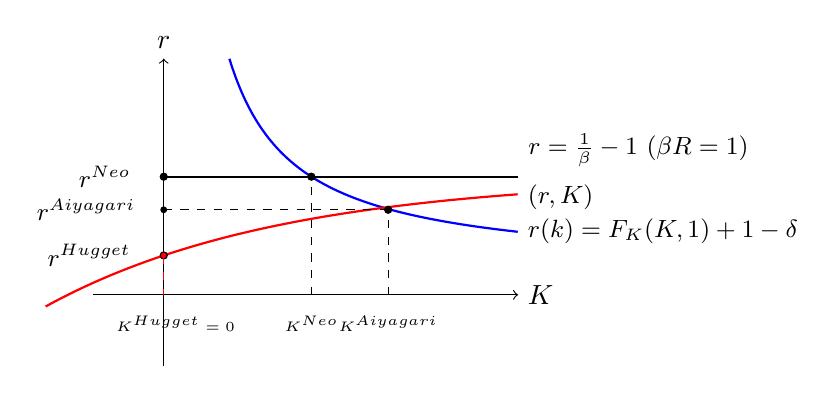
\begin{tikzpicture}[scale=3]
    % 绘制坐标轴
    \draw[->] (-0.3,0) -- (1.5,0) node[right] {$K$};
    \draw[->] (0,-0.3) -- (0,1) node[above] {$r$};
    
    % 线1：水平线 y = 0.5，标记为 1/\beta - 1
    \draw[black, thick] (0,0.5) -- (1.5,0.5) node[above right, font=\small] {$r = \frac{1}{\beta} - 1$ ($\beta R = 1$)};
    
    % 线2：双曲线 y = 2/(3x) + 0.2，限制在纵轴[0,1]范围内
    \draw[blue, thick] plot[smooth, domain=0.278:1.5, samples=100] (\x, {2/(8*\x) + 0.1});
    \node[right, font=\small] at (1.5, 0.267) {$r(k) = F_K(K,1)+1-\delta$};
    
    % 线3：曲线 y = -1/3*e^{-x} + 0.5
    \draw[red, thick] plot[smooth, domain=-0.5:1.5, samples=100] (\x, {-1/3 * exp(-\x) + 0.5});
    \node[above right, font=\small] at (1.5, 0.32) {$(r,K)$};
    
    % 标记1：黑色直线与y轴的交点 (0, 0.5)
    \draw[fill=black] (0,0.5) circle (0.015);
    \node[left, font=\small] at (-0.1, 0.5) {$r^{\text{Neo}}$};
    
    % 标记1b：黑色直线与蓝色曲线的交点 (约0.625, 0.5)
    \draw[fill=black] (0.625, 0.5) circle (0.015);
    % 横坐标标记
    \draw[dashed] (0.625, 0) -- (0.625, 0.5);
    \node[below, font=\tiny] at (0.625, -0.05) {$K^{\text{Neo}}$};
    
    % 标记2：红色曲线与y轴的交点 (0, 0.167)
    \draw[fill=red] (0,0.1667) circle (0.015);
    \node[left, font=\small] at (-0.1, 0.1667) {$r^{\text{Hugget}}$};
    % 虚线从交点延伸到原点
    \draw[dashed, red] (0,0.1667) -- (0,0);
    \node[below, font=\tiny] at (0.05, -0.05) {$K^{\text{Hugget}} = 0$};
    
    % 标记3：蓝色和红色曲线的交点（约在(0.95, 0.36)）
    \draw[fill=black] (0.95, 0.36) circle (0.015);
    % 纵坐标标记在y轴上
    \draw[fill=black] (0, 0.36) circle (0.012);
    \node[left, font=\small] at (-0.08, 0.36) {$r^{\text{Aiyagari}}$};
    % 虚线从y轴标记连接到交点
    \draw[dashed] (0, 0.36) -- (0.95, 0.36);
    % 横坐标标记
    \draw[dashed] (0.95, 0) -- (0.95, 0.36);
    \node[below, font=\tiny] at (0.95, -0.05) {$K^{\text{Aiyagari}}$};
\end{tikzpicture}
\end{center}


\begin{itemize}
    \item \textbf{The Blue Curve (Capital Demand):} This represents the firm's first-order condition, $r = F_K(K,1) - \delta$. It is downward-sloping due to the diminishing marginal product of capital. 
    \item \textbf{The Neo-classical Case (Complete Markets Benchmark):} In a standard representative-agent model (or with complete markets), there is no uninsurable idiosyncratic risk. The steady-state Euler equation is simply $1 = \beta (1+r)$, which completely and permanently pins down the interest rate at $r^{\text{Neo}} = \frac{1}{\beta} - 1$. Because the agent has no precautionary saving motive, the long-run asset supply curve is perfectly elastic (the horizontal black line). The equilibrium capital $K^{\text{Neo}}$ is strictly determined by where the firm's downward-sloping demand intersects this horizontal line.
    \item \textbf{The Red Curve (Incomplete Markets Asset Supply):} In the presence of uninsurable idiosyncratic risk, agents accumulate precautionary savings. As $r$ increases, the incentive to save grows, making the supply curve upward-sloping. Crucially, as $r \to \frac{1}{\beta} - 1$, agents become infinitely patient relative to the market return, and their asset demand diverges to infinity (as proven earlier via the supermartingale theorem). Thus, the red curve stays strictly below the black line and asymptotes to it.
    \item \textbf{The Huggett Case (Pure Exchange Economy):} In Huggett, there is no physical capital, meaning the net supply of assets must clear at exactly zero ($K=0$). The equilibrium interest rate $r^{\text{Huggett}}$ is found where the red supply curve intersects the y-axis. Notice that $r^{\text{Huggett}} < r^{\text{Neo}}$: to discourage agents from over-saving in a zero-net-supply economy, the market interest rate must be severely depressed.
    \item \textbf{The Aiyagari Case (Production + Incomplete Markets):} This is the grand synthesis. General equilibrium is reached at the intersection of the red savings supply curve and the blue capital demand curve. 
    \item \textbf{Key Takeaway (Aiyagari vs. Neo-classical):} Because the red supply curve strictly lies below the black line (due to precautionary savings), the Aiyagari intersection must occur further down the blue demand curve. Consequently, $K^{\text{Aiyagari}} > K^{\text{Neo}}$ and $r^{\text{Aiyagari}} < r^{\text{Neo}}$. The idiosyncratic risk forces agents to over-accumulate capital for self-insurance, which in turn drives down the equilibrium interest rate compared to the frictionless benchmark.
\end{itemize}
    
\defn{Stationary Equilibrium in Aiyagari Model}{
    A \textit{stationary equilibrium} consists of 
    \begin{itemize}
        \item stationary distribution: $\lambda(k,s)$,
        \item value function: $v(k,s)$,
        \item policy function: $k' = g(k,s)$, 
        \item prices: $r$ and $w(r)$,
        \item aggregate capital: $K$
        
    \end{itemize}
    such that
    \begin{itemize}
        \item Prices $r$ and $w(r)$ satisfy:
        \[
        \begin{aligned}
            w & = F_L(K,1),\\
            r &  = F_K(K,1) + 1-\delta.
        \end{aligned}
        \]
        \item $v(k,s)$ and $g(k,s)$ solve the agent's problem given $r$ and $w$.
        \item $\lambda(k,s)$ is the stationary distribution of $(k,s)$ given $g(k,s)$ and $\pi(s'|s)$:
        \[
        \lambda(k',s') = \sum_{s}\sum_{k:k' = g(k,s)}\pi(s'|s)\lambda(k,s).
        \]
        \item The stationary distribution $\lambda(k,s)$ and policy function $g(k,s)$ generate aggregate capital $K$:
        \[
        \sum_k\sum_s g(k,s)\lambda(k,s) = K.
        \]
    \end{itemize}
}

\state{Algorithm for Aiyagari Model Solution}{
    \begin{enumerate}
        \item Guess an aggregate capital $K_0$.
        \item Obtain the prices $r$ and $w$ from the firm's first-order conditions:
        \[
        \begin{aligned}
            r & = F_K(K_0,1) + 1-\delta,\\
            w & = F_L(K_0,1).
        \end{aligned}
        \]
        \item Solve the agent's recursive problem to obtain the policy function $k' = g(k,s)$.
        \item Obtain the stationary distribution $\lambda(k,s)$.
        \item Update $K_0$ by $K_1$\footnote{
            A more robust way to update $K$ is to use a convex combination of $K_0$ and $K_1$: $K^* = \ve K_0 + (1-\ve)K_1$, where $\ve\in (0,1)$ is called the relaxation parameter.
        }:
        \[
        K_1 = \sum_k\sum_s g(k,s)\lambda(k,s).
        \]
        \item Iterate until $K_0 = K_1$.
    \end{enumerate}
}

\section{Krusell-Smith Model}

\rmk{
Both the Huggett and Aiyagari models are steady-state models. While individuals experience idiosyncratic shocks and their personal wealth fluctuates, the \textit{aggregate} economy never changes. There are no business cycles, and the wealth distribution $\lambda(k,s)$ is perfectly stationary. Prices ($r$ and $w$) remain constant forever. The Krusell-Smith (1998) model breaks this tranquility by introducing \textbf{Aggregate Shocks} (e.g., TFP shocks, $z_t$). This seemingly innocent addition creates a massive technical nightmare:
\begin{itemize}
    \item \textbf{Fluctuating Prices:} Because TFP fluctuates, aggregate capital $K_t$ and labor demand fluctuate, meaning $r_t$ and $w_t$ now change over time.
    \item \textbf{The Curse of Dimensionality:} To make an optimal saving decision today, an agent must forecast tomorrow's prices ($r_{t+1}, w_{t+1}$). To forecast tomorrow's prices, they must forecast tomorrow's aggregate capital $K_{t+1}$. But $K_{t+1}$ depends on how \textit{everyone} in the economy saves today. Therefore, the agent must know the \textbf{entire current wealth distribution $\lambda_t$} to predict the future. 
    \item \textbf{The Infinite-Dimensional State Space:} The distribution $\lambda_t$ is an infinite-dimensional object. Putting an infinite-dimensional object into a Bellman equation as a state variable makes it computationally impossible to solve using traditional grid methods.
\end{itemize}
}

Assume:
\begin{itemize}
    \item Aggregate shock $z_t$ to productivity such that
    \[
    y_t = z_t F(K_t,L_t).
    \]
    \begin{itemize}
        \item Assume $z_t$ follows a finite-state Markov process.
        \item $z_t$ can be interpreted as an aggregate technology (business cycle) shock.
    \end{itemize}
    \item Idiosyncratic shock $s_t$ to labor productivity (also a Markov process).
\end{itemize}

Therefore, the agents' wealth will depend on both the aggregate shock $z_t$ and the idiosyncratic shock $s_t$. Pay special attention to the fact that the aggregate distribution $\lambda_t$ will now vary over time depending on the realization of $z_t$.

The recursive problem of the agent is given by
\[
\begin{aligned}
    v(k,s,\lambda, z) & = \max_{c,k'} u(c) + \beta \mathbb E\br{v(k',s',\lambda', z')|s,\lambda,z}\\
\text{s.t. } & c + k' \le \pr{r(\lambda,z)+1-\delta}k + w(\lambda,z)l(s),\\
& \lambda' = H(\lambda, z,z').
\end{aligned}
\]
where $\lambda$ is the distribution of capital across agents, and $H(\cdot)$ is the highly complex aggregate law of motion for the distribution of capital. Notice that prices $r$ and $w$ are now explicitly functions of the aggregate state $(\lambda, z)$.

From the Bellman equation, we can obtain the policy function for capital $k' = g(k,s,\lambda,z)$ by combining the budget constraint and the law of motion for capital.

In the aggregate, the market clearing condition is
\[
K_t = \int k\lambda_t(k,s)\d k\d s.
\]

\defn{Recursive Competitive Equilibrium}{
    A \textit{recursive competitive equilibrium} consists of
    \begin{itemize}
        \item value function $v(k,s,\lambda,z)$,
        \item policy function $k' = g(k,s,\lambda,z)$,
        \item pricing functions $r(\lambda,z)$ and $w(\lambda,z)$, and
        \item Aggregate law of motion $H$ that maps $(\lambda, z, z')$ to $\lambda'$ 
    \end{itemize}
    such that 
    \begin{itemize}
        \item \textbf{Individual Optimization:} Given $H$, $r$, and $w$, the functions $v$ and $g$ solve the agent's Bellman equation.
        \item \textbf{Firm Optimization:} Prices satisfy the firm's first-order conditions: $r(\lambda,z) = z F_K(K,L) - \delta$ and $w(\lambda,z) = z F_L(K,L)$.
        \item \textbf{Market Clearing:} Aggregate capital equals the sum of all individual asset holdings:
        \[
        K = \int k \d\lambda(k,s).
        \]
        \item \textbf{Consistency (Rational Expectations):} The perceived aggregate law of motion $H$ is consistent with the actual law of motion generated by the aggregation of individual policy functions $g$:
        \[
        \lambda'(k',s') = \int \int_{k'=g(k,s,\lambda,z)} \pi(s'|s) \pi(z'|z) \d\lambda(k,s).
        \]
    \end{itemize}
}

\state{Algorithm for Krusell-Smith Model Solution}{
    \begin{enumerate}
        \item Characterize $\lambda(k,s)$ by a finite number of moments: $m = \brace{m_1,m_2,\cdots,m_I}$.
        \item Assume a functional form for $H$ that maps $m$ to $m'$: $m' = H(m,z,z')$.
        \item Guess the $m$'s and $H$.
        \item Solve the Bellman equation to obtain the value function $v(k,s,m,z)$ and the policy function $k' = g(k,s,m,z)$.
        \item Simulate the economy:
        \begin{itemize}
            \item Draw realizations for $\brace{z_t}_{t=  0}^T$.
            \item Simulate the paths of $\brace{s_t}_{t=0}^T$ for a large number of agents.
            \item Obtain the simulated paths of $\brace{k_t}_{t=0}^T$ for each agent by using the policy function $g(k,s,m,z)$.
            \item Assemble the simulated paths of $k_t$ to obtain the simulated paths of $m_t$.
        \end{itemize}
        \item Update $H$ based on the simulated paths of $m_t$.
        \item Iterate until convergence.
        \end{enumerate}
}

\rmk{
    It turns out that tracking only the first moment ($m_1 = K$) is spectacularly sufficient! The $R^2$ of the forecasting regression $\ln K' = a_z + b_z \ln K$ is typically above 0.999. Why does this ``Approximate Aggregation" work so perfectly? 
    
    The intuition lies in the shape of the policy functions. The poorest agents face binding borrowing constraints, so their saving policy function is highly non-linear. However, the poorest agents hold almost zero capital, so their non-linear behavior barely moves the macroeconomic aggregate $K$. Conversely, the richest agents hold the vast majority of the economy's capital. For these wealthy agents, the precautionary saving motive is negligible, and their saving policy function $k' = g(k,\dots)$ is almost perfectly linear with respect to $k$. 
    
    Since the people who actually matter for the aggregate sum behave linearly, the aggregate capital tomorrow ($K'$) simply depends on the aggregate capital today ($K$), completely ignoring how that capital is distributed among the rich. Thus, the infinite-dimensional distribution $\lambda$ elegantly collapses back into a single number $K$.
}

